\section{700 MHz densification}
%\subsection*{700 MHz densification}
%\addcontentsline{toc}{subsection}{700 MHz densification}
700 MHz densification is the new intervention created in this Master Thesis. It consists in integrating the 700 MHz band in the existing base stations in the area and, once all of them have 700 MHz carriers, the intervention builds new base stations until the capacity demanded is reached, the coverage obligations are fulfilled, or the maximum site density is reached.\par

After that, I have created a new capacity expansion strategy, the �\textit{700 MHz densification�} that is only allowed to use the �\textit{700 MHz densification�} strategy.\textit{ }The following figures show the effects that using this capacity strategy has on the development of the mobile telecommunications network. \par

\subsection*{Investment}
%\addcontentsline{toc}{subsection}{Investment}
The cost distribution is the first of the two most important outputs to analyse of a simulation. The investment graph shows the evolution of the investment over the years and produces several important results: (i) It allows to check how much it has been spent per year, (ii) how many years the telecom operator exhausted all its budget, (iii) when the capacity cannot be further increased because it has reached the limit of the technology. \par

The following graph represents the investment made by the telecom operator per year to build new assets in all the country. The green line shows in which year the telecom operator starts to invest to satisfy the demand instead of investing to fulfil the coverage obligations. This test uses the baseline population growth scenario, the baseline user-speed growth scenario, and the \textit{�More profitable first�} coverage obligation option with a speed of 2 Mbps. \par



%%%%%%%%%%%%%%%%%%%% Figure/Image No: 2 starts here %%%%%%%%%%%%%%%%%%%%

\begin{figure}[H]
	\begin{Center}
		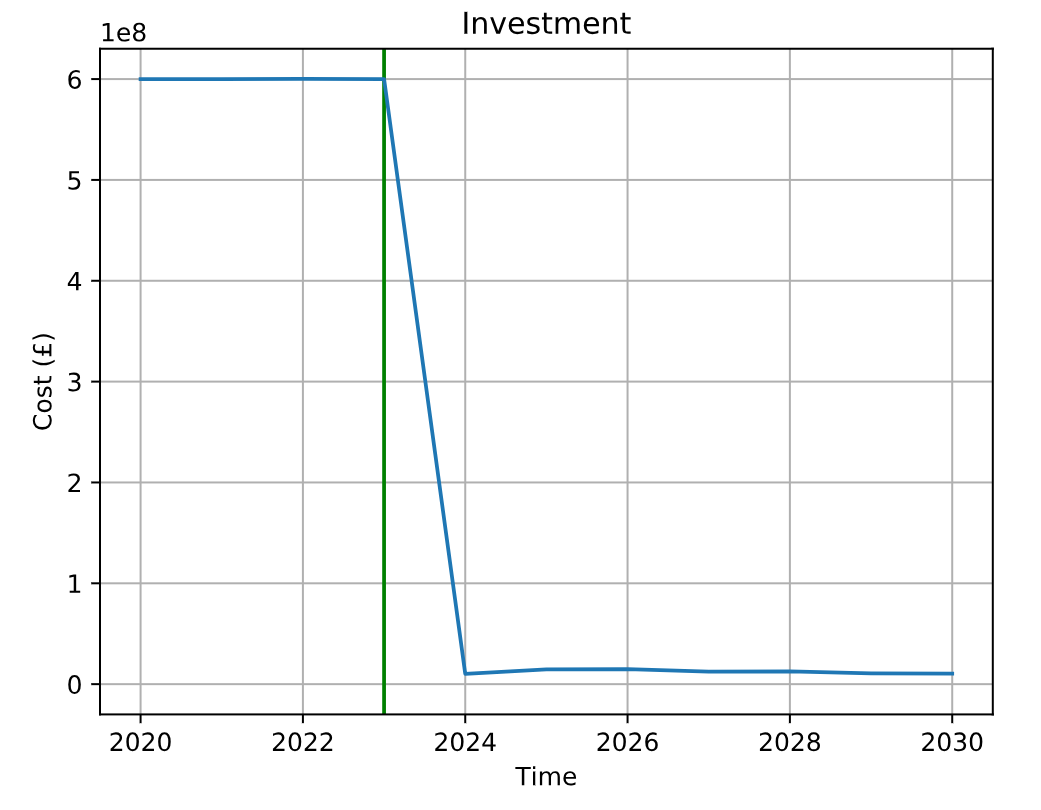
\includegraphics[width=0.85\textwidth]{./media/image41.png}
		\caption{700 MHz densification. Graph: Investment. Source: Author}
	\end{Center}
\end{figure}


%%%%%%%%%%%%%%%%%%%% Figure/Image No: 2 Ends here %%%%%%%%%%%%%%%%%%%%

As it can be seen, the investment is not the same every year. For the first 4 years (from 2020 to 2023) the telecom operator invests all the budget that it has: around �600,000,000. In the year 2023 the investment rate decreases to less than 10$\%$  of the maximum, two things could happen: (i) the telecom operator determines that is fulfilling the coverage obligations and stops investing, (ii) despite some regions still need more investment, it is not possible due to technical limitations. We need the population covered analysis to determine which is the case.\par

Another output that is important is the cost of increasing the population covered using this strategy. It is not linear since each geotype have different propagation characteristics. The following graph shows information related to this output:\par



%%%%%%%%%%%%%%%%%%%% Figure/Image No: 3 starts here %%%%%%%%%%%%%%%%%%%%

\begin{figure}[H]
	\begin{Center}
		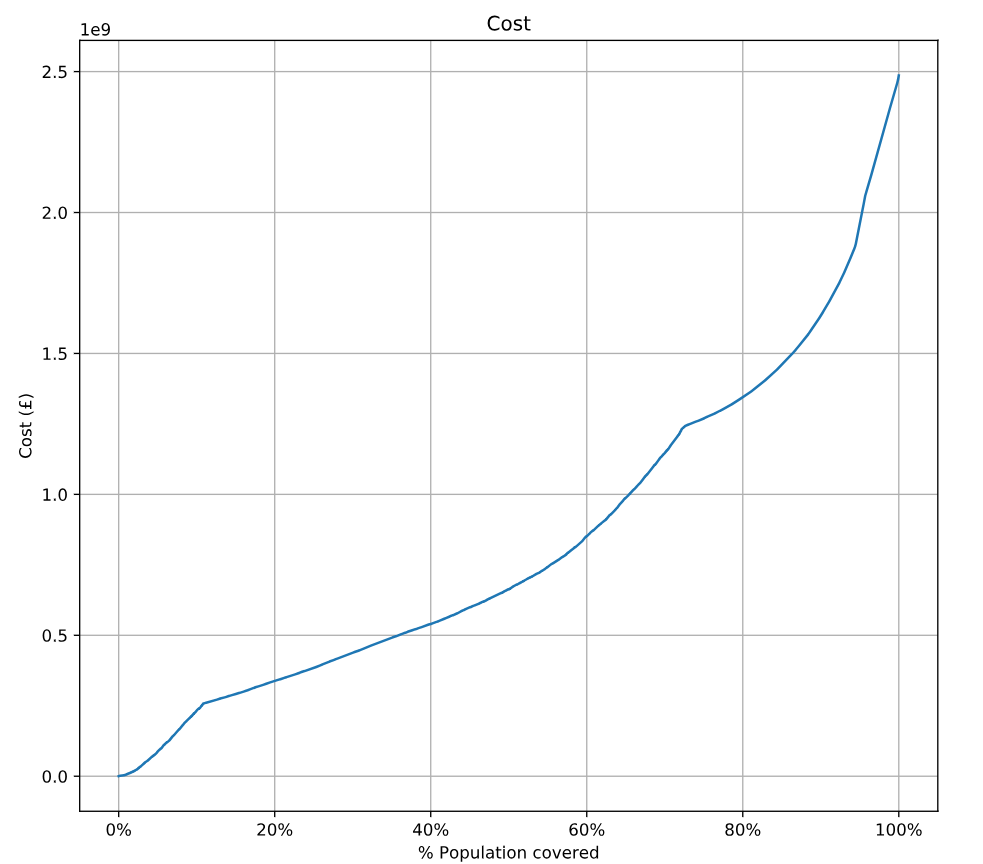
\includegraphics[width=0.95\textwidth]{./media/image42.png}
		\caption{700 MHz densification. Graph: Cost. Source: Author}
	\end{Center}
\end{figure}


%%%%%%%%%%%%%%%%%%%% Figure/Image No: 3 Ends here %%%%%%%%%%%%%%%%%%%%

This test uses the baseline population growth scenario, the baseline user-speed growth scenario, and the \textit{�More profitable first�} coverage obligation option with a speed of 2 Mbps. The graph represents the cumulative costs of having a certain percentage of population covered. It shows an increasing growth of the marginal costs as the coverage increases. The reason is that \textit{�More profitable first�} orders all the PCDs from most to least densely populated, which means that urban PCDs are first and rural PCDs are the last.\par

There are three main parts in which rates of cost increase could be divided: (i) Urban areas (circa 0$\%$  to 10$\%$ ), (ii) suburban areas (circa 10$\%$  to 75$\%$ ), and (iii) rural areas (circa 75$\%$  to 100$\%$ ). Despite the slope of the curve is not constant inside each part, in general terms, the slope is steeper for the rural areas because the population density is so low that the operator has to add ever more antennas. This is not because of capacity needs, but because of the limitation in range of coverage due to the attenuation losses. On the contrary, in highly populated areas, the operator is forced to build a lot of assets, because it needs a lot of capacity, but this strategy raises the costs significantly.\par

Finally, the following coloured map represents the distribution of costs across the country and how the most populated areas, especially London area, receive more investments during all the years:\par



%%%%%%%%%%%%%%%%%%%% Figure/Image No: 4 starts here %%%%%%%%%%%%%%%%%%%%

\begin{figure}[H]
	\begin{Center}
		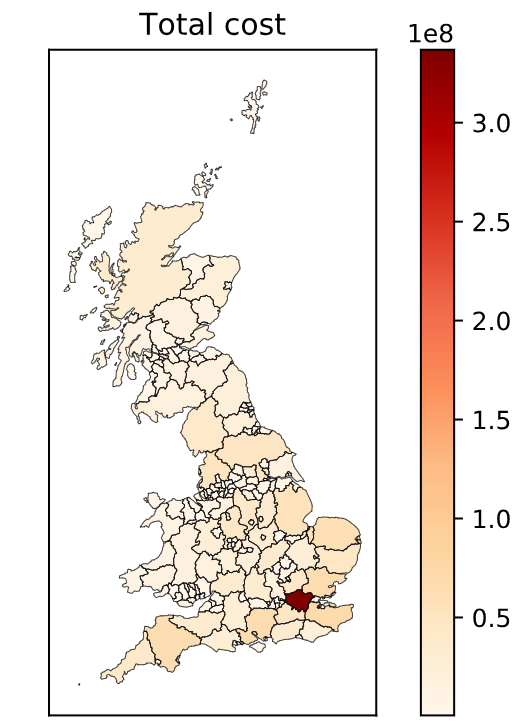
\includegraphics[width=0.65\textwidth]{./media/image43.png}
		\caption{700 MHz densification. Map: Total cost. Source: Author}
	\end{Center}
\end{figure}


%%%%%%%%%%%%%%%%%%%% Figure/Image No: 4 Ends here %%%%%%%%%%%%%%%%%%%%

\subsection*{Population covered}
%\addcontentsline{toc}{subsection}{Population covered}
The population covered over time is the second most important outputs to analyse. The detail per year produces three important results: (I) How the population is covered year by year, (II) If the given run is good enough to satisfy the demand and the coverage obligations in ten years, (III) If there are regions that simply cannot have enough capacity due to several reasons. The following map shows the evolution over time of the percentage of users that have at least the 2Mbps that the coverage obligation forces:\par



%%%%%%%%%%%%%%%%%%%% Figure/Image No: 5 starts here %%%%%%%%%%%%%%%%%%%%

\begin{figure}[H]
	\begin{Center}
		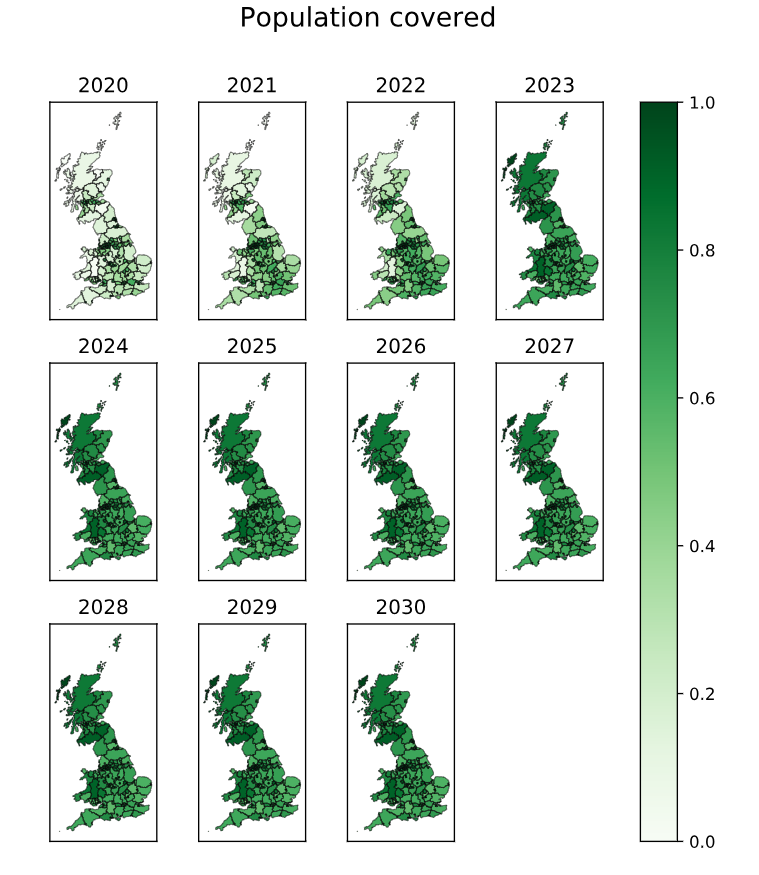
\includegraphics[width=0.95\textwidth]{./media/image44.png}
		\caption{700 MHz densification. Map: Population covered. Source: Author}
	\end{Center}
\end{figure}


%%%%%%%%%%%%%%%%%%%% Figure/Image No: 5 Ends here %%%%%%%%%%%%%%%%%%%%

This map only shows information at a LAD level, but this information will be covered in higher detail in the following graphs. This test uses the baseline population growth scenario, the baseline user-speed growth scenario, and the \textit{�More profitable first�} coverage obligation with a speed of 2 Mbps.\par

As it can be seen, most of the regions do not have enough capacity installed in the beginning and the most populated regions (those that have a bigger percentage) had a larger percentage of population covered. This is where telecom operators normally invest because it is generally more profitable (As the population density is higher, people concentrate in bigger cities and telecom operators can reach more people just with one base station).\par

With this capacity expansion strategy, coverage growths quickly at first, while from 2023 to 2030 it remains approximately similar. The final percentage is considerably better than at the beginning, but it is not 100$\%$  in all the regions. The following histogram shows the distribution of the coverage obligation percentage at the end with a higher detail since it represents the probability of a PCD of having a specific population covered percentage:\par



%%%%%%%%%%%%%%%%%%%% Figure/Image No: 6 starts here %%%%%%%%%%%%%%%%%%%%

\begin{figure}[H]
	\begin{Center}
		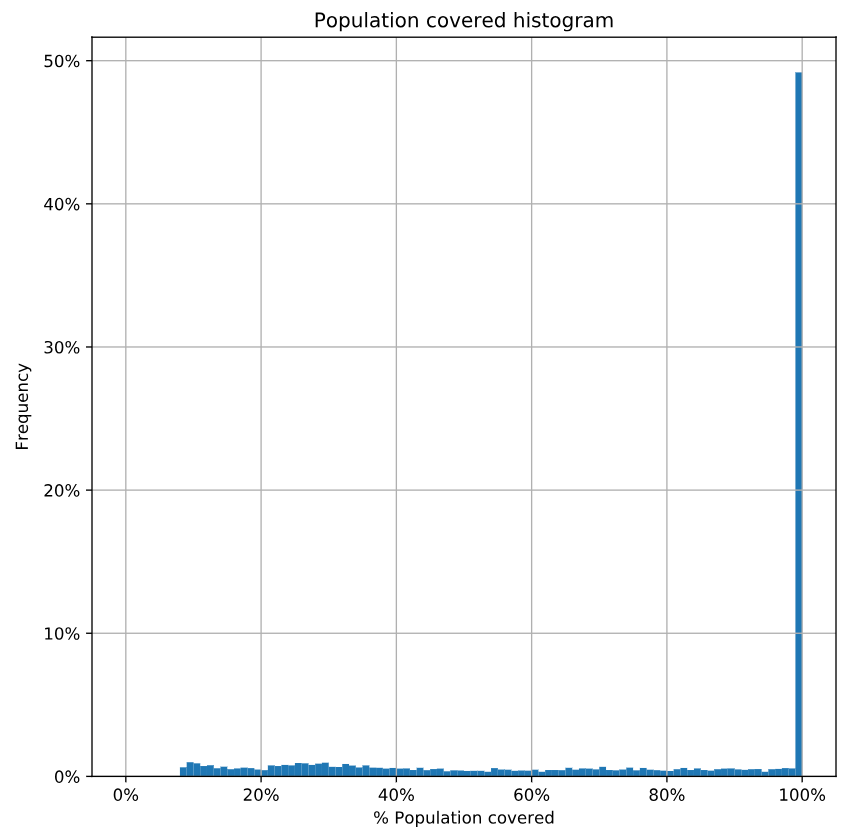
\includegraphics[width=0.80\textwidth]{./media/image45.png}
		\caption{700 MHz densification. Histogram: Population covered. Source: Author}
	\end{Center}
\end{figure}


%%%%%%%%%%%%%%%%%%%% Figure/Image No: 6 Ends here %%%%%%%%%%%%%%%%%%%%

This test uses the baseline population growth scenario, the baseline user-speed growth scenario, and the \textit{�More profitable first�} coverage obligation option with a speed of 2 Mbps. As it can be seen in the histogram, almost half of the PCDs fulfil their coverage obligations completely, but the other half cannot.\par

Combining the results of the histogram with the investment per year graph, it can be inferred that the telecom operator has enough budget to continue with the investments, but it cannot due to technical limitations. In this case, the telecom operator can only use the 700 MHz band and its capacity is limited. Half of the PCDs demand less than the maximum capacity of the band and the rest have only a portion of the coverage obligation fulfilled.\par

\subsection*{Technology upgrades}
%\addcontentsline{toc}{subsection}{Technology upgrades}
The code also allows one to see the technology upgrades of every region of the country. The following chart represents the technology upgrades made using the 700 MHz intervention. It uses the baseline population growth scenario, the baseline user-speed growth scenario, and the \textit{�More profitable first�} coverage obligation with a speed of 2 Mbps. As can be seen, the distribution of the deployment of base stations is not homogeneous since the London region is much more populated than areas from Wales or Scotland.\par



%%%%%%%%%%%%%%%%%%%% Figure/Image No: 7 starts here %%%%%%%%%%%%%%%%%%%%

\begin{figure}[H]
	\begin{Center}
		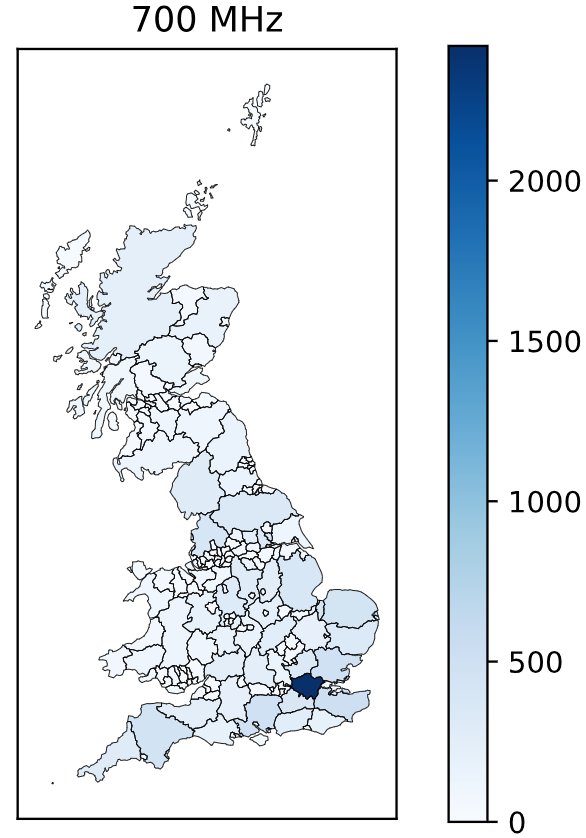
\includegraphics[width=0.50\textwidth]{./media/image46.png}
		\caption{700 MHz densification. Map: Technology upgrades. Source: Author}
	\end{Center}
\end{figure}


%%%%%%%%%%%%%%%%%%%% Figure/Image No: 7 Ends here %%%%%%%%%%%%%%%%%%%%

\subsection*{Capacity margin}
%\addcontentsline{toc}{subsection}{Capacity margin}
The section �Population Covered� discussed the\ relation between the capacity installed and the coverage obligation. Now, we study the capacity and demand parameters and its relation, the capacity margin.  The following coloured map represents the evolution of the capacity along the years.\par



%%%%%%%%%%%%%%%%%%%% Figure/Image No: 8 starts here %%%%%%%%%%%%%%%%%%%%

\begin{figure}[H]
	\begin{Center}
		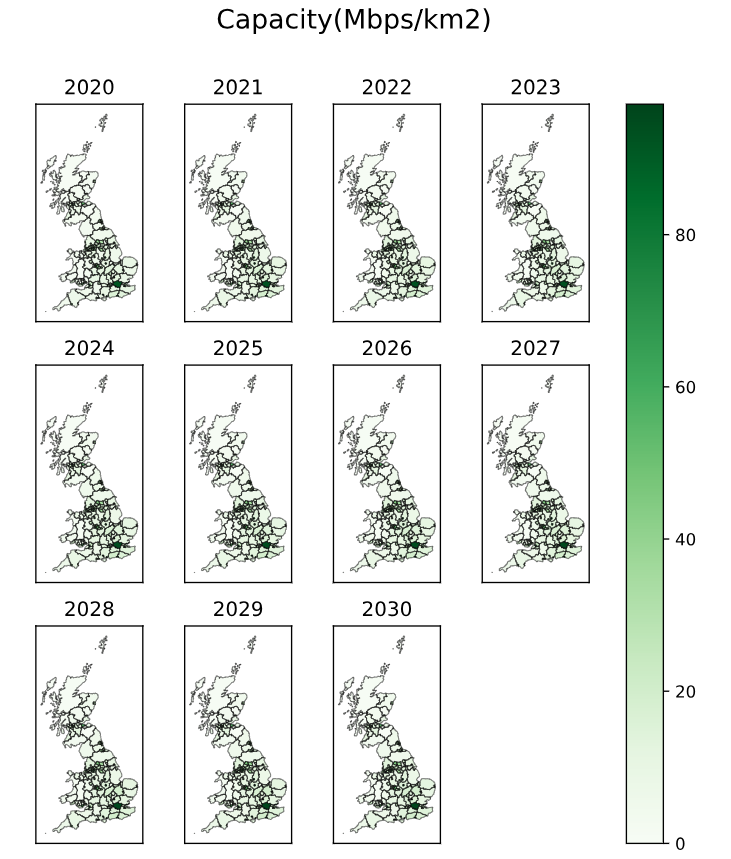
\includegraphics[width=0.9\textwidth]{./media/image47.png}
		\caption{700 MHz densification. Map: Capacity evolution. Source: Author}
	\end{Center}
\end{figure}


%%%%%%%%%%%%%%%%%%%% Figure/Image No: 8 Ends here %%%%%%%%%%%%%%%%%%%%

This map is calculated using the baseline population growth scenario, the baseline user-speed growth scenario, and the \textit{�More profitable first�} coverage obligation with a speed of 2 Mbps. It represents the capacity in Mbps per km\textsuperscript{2} installed at the end of each year and allows to see the evolution of the investment but also to see how much capacity was installed in each region at the beginning of the simulation. Note that if the reader wants to back-calculate the maximum population that could be satisfied using a capacity of 50 Mbps per km\textsuperscript{2} the conversion is not direct since they should consider the overbooking factor, the market share of the operator, etc. The following map represents the evolution of the demand over the years using the same simulation:\par



%%%%%%%%%%%%%%%%%%%% Figure/Image No: 9 starts here %%%%%%%%%%%%%%%%%%%%

\begin{figure}[H]
	\begin{Center}
		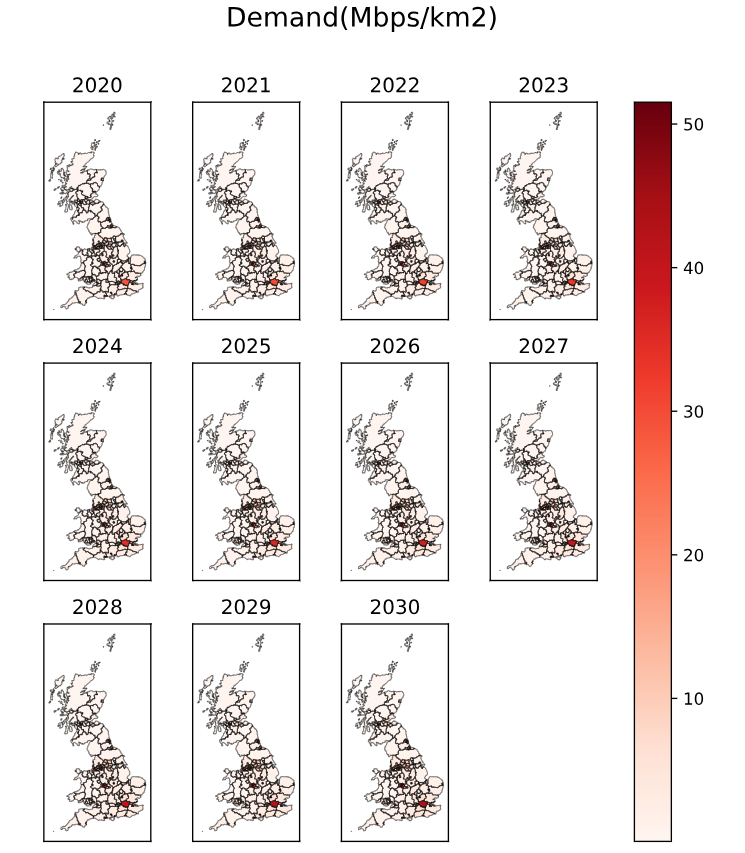
\includegraphics[width=0.90\textwidth]{./media/image48.png}
		\caption{700 MHz densification. Map: Demand evolution. Source: Author}
	\end{Center}
\end{figure}


%%%%%%%%%%%%%%%%%%%% Figure/Image No: 9 Ends here %%%%%%%%%%%%%%%%%%%%

Finally, the following coloured map calculates the subtraction of the demand from the capacity values and represents the amount of capacity in Mbps per km\textsuperscript{2} that each region lacks or has extra. This is the value that, without coverage obligations, the telecom operators normally use to check which are the highest priority areas to invest.\par


%%%%%%%%%%%%%%%%%%%% Figure/Image No: 10 starts here %%%%%%%%%%%%%%%%%%%%

\begin{figure}[H]
	\begin{Center}
		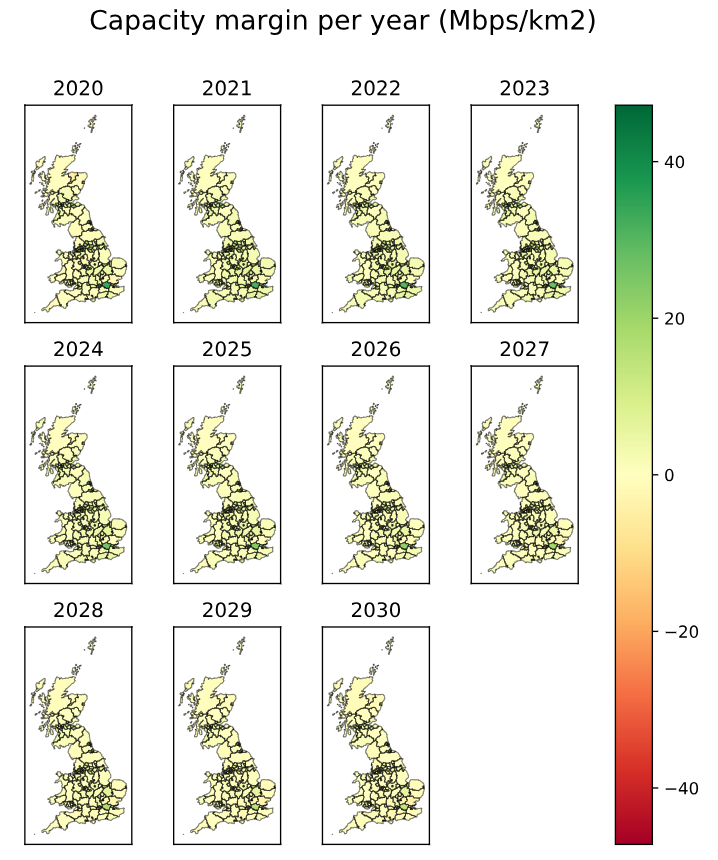
\includegraphics[width=0.90\textwidth]{./media/image49.png}
		\caption{700 MHz densification. Map: Capacity margin evolution. Source: Author}
	\end{Center}
\end{figure}


%%%%%%%%%%%%%%%%%%%% Figure/Image No: 10 Ends here %%%%%%%%%%%%%%%%%%%%
\subsection*{Total costs}
%\addcontentsline{toc}{subsection}{Total costs}
The previous analysis was executed considering that the telecom operator has a limited amount of money available to invest every year. As we want to be sure if the operator is limited by investment force or technical requirements, I have run a new execution of the code without limits in the annual budget and the results are the same. The problem of using only the 700 MHz band is that telecom operators cannot satisfy the demand.\par
